% ------------------------------------------------------------------------------
%
% PREAMBLE
%
% ------------------------------------------------------------------------------

\documentclass[12pt, titlepage]{article}


\usepackage{graphicx, amsmath, amssymb, natbib, setspace, sectsty, verbatim, 
		mathrsfs, float}
\usepackage{MnSymbol}
\usepackage{multirow}
\usepackage{bm}
\usepackage[usenames, dvipsnames]{color}
\bibpunct{(}{)}{;}{a}{}{,}
\setlength{\parindent}{3em}
%\parskip = 1.5ex
%\linespread{1.3}
%\onehalfspacing

\pdfpagewidth 8.5in
\pdfpageheight 11in
\setlength{\oddsidemargin}{0.0in} \setlength{\textwidth}{6.5in}
\setlength{\topmargin}{0.15in} \setlength{\textheight}{8.5in}
\setlength{\headheight}{0.0in} \setlength{\headsep}{0.0in}

\usepackage{/mnt/ExtraDrive1/Work/shTex/mymacros}

\providecommand{\norm}[1]{\lVert#1\rVert}
\newcommand{\csection}[1]{\section[#1]{\centering #1 }}
\subsectionfont{\small}
\newcommand{\cye}[1]{\color{yellow!70!black}#1}
\newcommand{\cre}[1]{\color{red!70!black}#1}
\newcommand{\cbl}[1]{\color{blue!70!black}#1}
\newcommand{\cgr}[1]{\color{green!70!black}#1}


% ------------------------------------------------------------------------------
%
% BEGIN DOCUMENT
%
% ------------------------------------------------------------------------------

\begin{document}

\setcounter{equation}{0}
\renewcommand{\theequation}{R.\arabic{equation}}


% ------------------------------------------------------------------------------
%
%                    Section 8.8.1
%                    Seal trend data
%
% ------------------------------------------------------------------------------

{\large \flushleft \textbf{8.8.4 Moss Heavy Metal Data}}

\vspace{.3cm}

In Section 4.5.4, we used a linear model for the logarithm (base $e$) of lead (Pb) concentration in tissue samples that included explanatory variables for 1) year of sample (2001 or 2006), 2) (log, base $e$) distance-from-road, and 3) side-of-road (north or south), and up to a 3-way interaction between these effects.  Here we will allow for spatially-autocorrelated errors, and random effects that accommodate the special sampling design of this study.  

The spatial sampling design affects how efficiently we estimate autocorrelation, how well we estimate fixed effects, and how precise we predict at unsampled locations.  These issues will be discussed in greater detail in Chapter 10.  However, intuitively, it should make sense that in order to estimate autocorrelation well, we should have some pairs of sample locations that are very close together, as that will help us estimate autocorrelation at short distances and anchor the autocovariance functions introduced in Chapter 6.  This idea was used for the moss heavy metal data, although it is not apparent from the earlier figures (e.g., Figure 1.8).  Figure~\ref{Fig:MossACsamples}A shows the Cape Krusenstern study area with all samples from 2001, and notice the shaded rectangular box within the study area.  This rectangular box is expanded in Figure~\ref{Fig:MossACsamples}B.  The primary sample units are show as $+$ symbols, which were targeted for a certain vegetation class and then randomized within strata , where strata were determined by distance from the haul road.  At some of the primary sites, ``autocorrelation'' sites were established, which were sampled random directions and distances between 10 and 20 meters from the primary sites.  The autocorrelation sites are shown with $\times$ symbols (Figure~\ref{Fig:MossACsamples}B).

At some locations, duplicate samples were taken. That is, we are interested in the microscale variation due to grabbing one handful of moss versus reaching over and grabbing a different handful of moss. In terms of our spatial autocorrelation matrix, these samples will have a distance of zero, which causes correlation of 1 for off-diagonal elements of the covariance matrix.  These off-diagonal 1's can cause that matrix to be non-positive definite, and computer algorithms for inverses, determinants, etc., may be unstable.  However, if we add a random effect for location, which adds a variance term for repeatedly sampling a single location, the non-positive definite matrix issue gets resolved.  So let $\mathbf{Z}_{1}$ be a design matrix of dummy variables (ones and zeros) that indicate at which location a sample occurs. 

Additionally, moss samples are sent to a laboratory for analysis of Pb concentration.  The process of extracting the heavy metal, and then measuring it by a machine may have what is sometimes termed ``measurement error.''  In order to assess measurement error, after moss samples were homogenized, some of the homogenized samples were split into two and both were run through the heavy metal extraction and concentration measurement.  We let $\mathbf{Z}_{2}$ be a design matrix of dummy variables that label laboratory replicates that are nested within the location and possibly a duplicate sample for a location as described in the previous paragraph.

\begin{figure}[H]
  \begin{center}
	    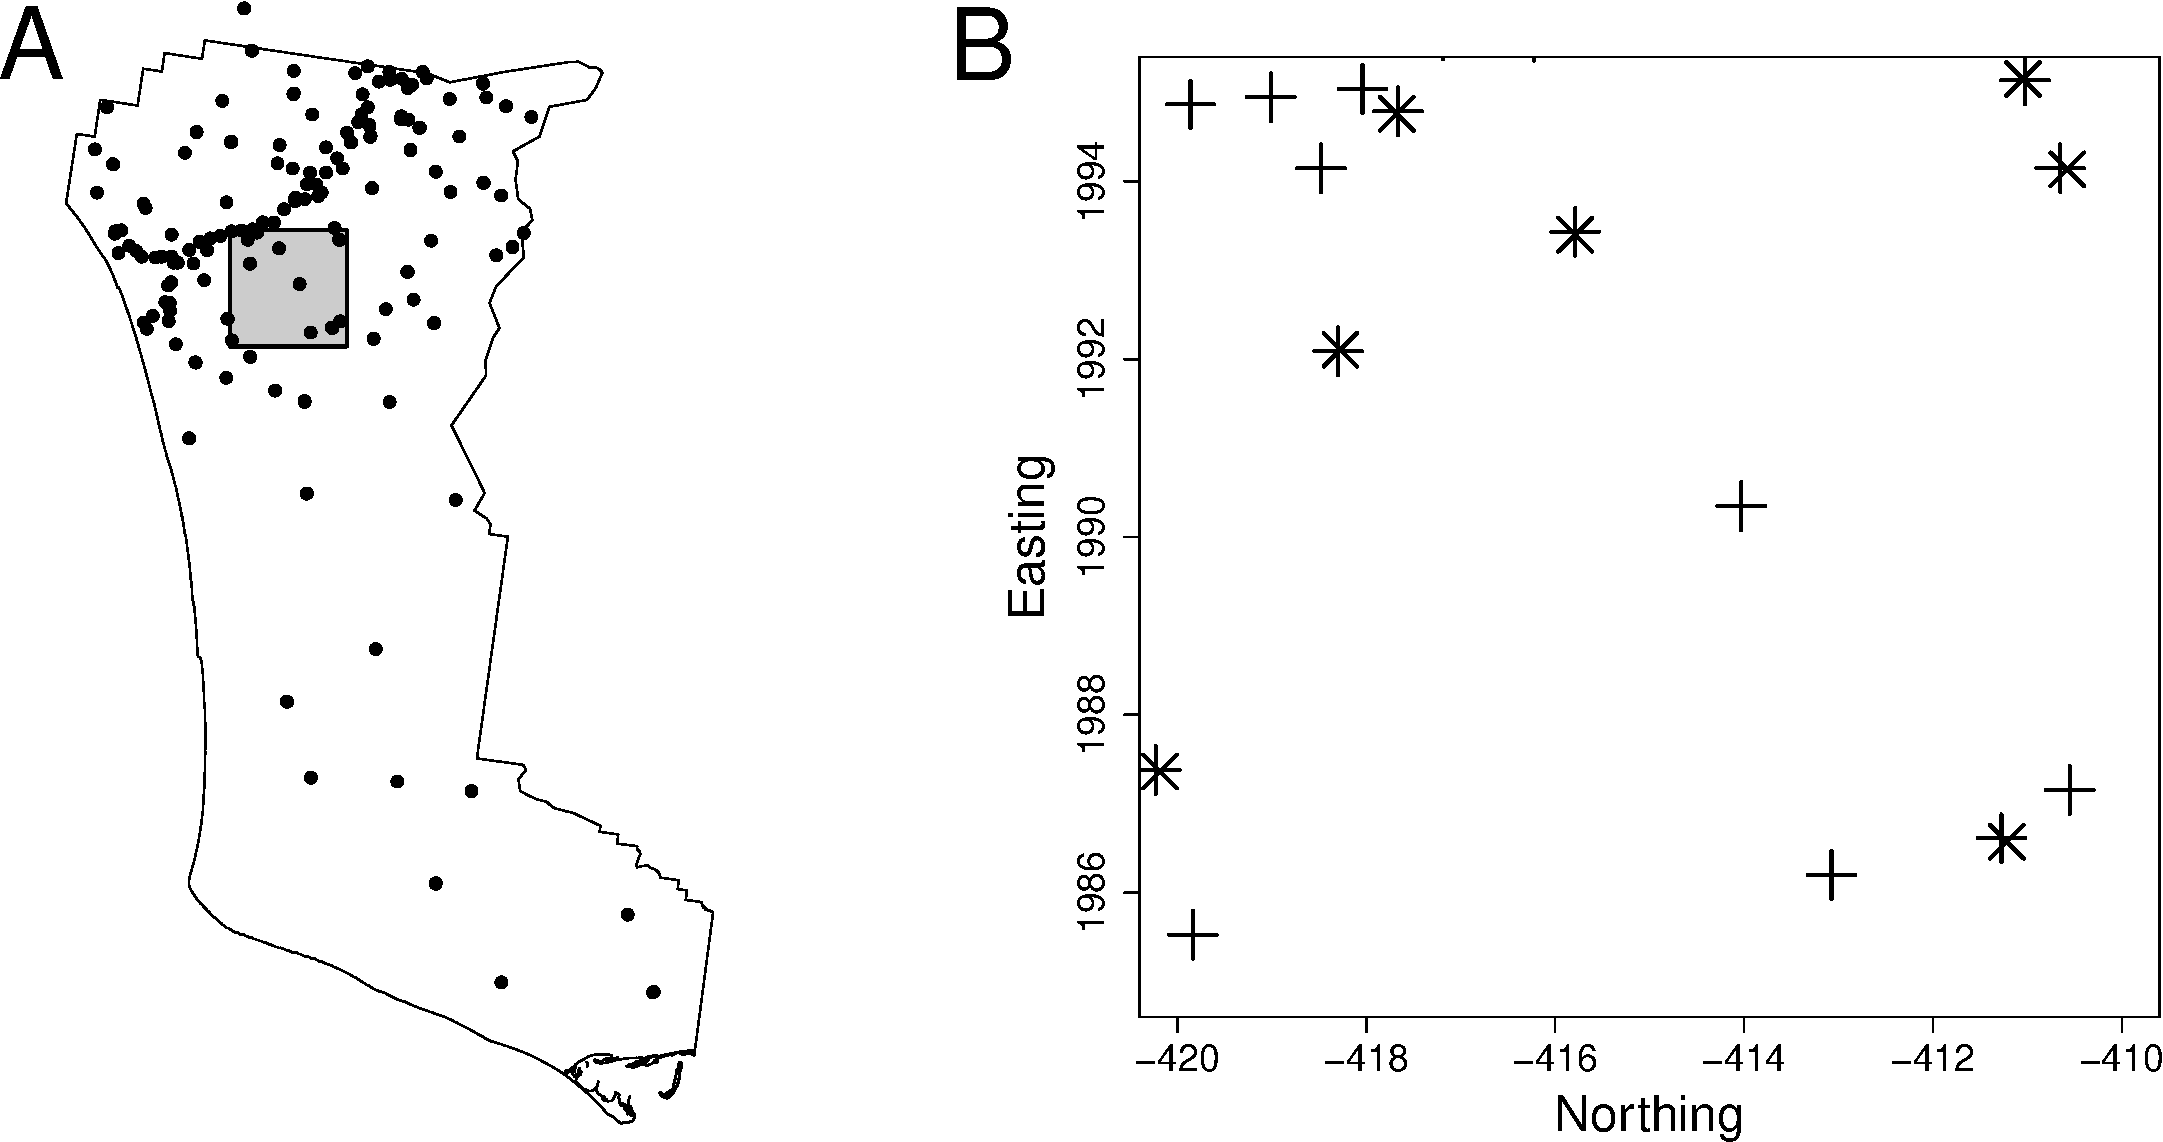
\includegraphics[width=0.9\linewidth]{Moss_autocorr_samples}
  \end{center}
  \caption{Sampling locations from 2001. A. Cape Krusenstern study area. B.  The shaded rectangular box in the study area has been expanded showing primary sampling locations ($+$) and autocorrelation sampling locations ($\times$).  \label{Fig:MossACsamples}}
\end{figure}

The covariance matrix resulting from the sampling design above can be illustrated with a simple example of 3 locations, where location 1 is far from locations 2 and 3 (say autocorrelation of 0.01), but site 3 is an autocorrelation location for site 2 (say autocorrelation of 0.99).  Additionally, suppose that site 2 had two duplicate samples (nested within sites), and for each duplicate sample, there were two laboratory replicate samples, for a total of 6 samples.  Then
$$
\mathbf{Z}_{1} = \left(
\begin{array}{ccc}
	1 & 0 & 0 \\
	0 & 1 & 0 \\
	0 & 1 & 0 \\
	0 & 1 & 0 \\
	0 & 1 & 0 \\
	0 & 0 & 1 \\
\end{array}
\right) 
\hspace{.5 cm} \textrm{and} \hspace{.5cm} 
\mathbf{Z}_{2} = \left(
\begin{array}{cccc}
	1 & 0 & 0 & 0 \\
	0 & 1 & 0 & 0 \\
	0 & 1 & 0 & 0 \\
	0 & 0 & 1 & 0 \\
	0 & 0 & 1 & 0 \\
	0 & 0 & 0 & 1 \\
\end{array}
\right), 
$$
and notice that laboratory replicates, nested within site and duplicate samples, will result in a diagonal matrix, so it is confounded with the nugget effect, which is appropriate, because for this model we consider the nugget effect to be measurement error.  Let $\sigma^{2}_{PS}$ be the variance (partial sill) for the spatial autocorrelation matrix $\mathbf{R}$, let $\sigma^{2}_{LO}$ be the variance of the random effect for location, let $\sigma^{2}_{DU}$ be the variance of the random effect for duplicate samples per location, and let $\sigma^{2}_{ME}$ be the variance due to laboratory measurement errors (nugget effect).  The resulting covariance is
$$
\boldsymbol{\Sigma} = \sigma^{2}_{PS}\mathbf{R} + \sigma^{2}_{LO}\mathbf{Z}_{1}\mathbf{Z}_{1}^{T} + \sigma^{2}_{DU}\mathbf{Z}_{2}\mathbf{Z}_{2}^{T} + \sigma^{2}_{ME}\mathbf{I},
$$
and for the simple example with 3 locations and 6 samples,
$$
\begin{array}{c}
\boldsymbol{\Sigma} = \sigma^{2}_{PS}\left(
\begin{array}{cccccc}
	1 & 0.01 & 0.01 & 0.01 & 0.01 & 0.01 \\
	0.01 & 1 & 1 & 1 & 1 & 0.99 \\
	0.01 & 1 & 1 & 1 & 1 & 0.99 \\
	0.01 & 1 & 1 & 1 & 1 & 0.99 \\
	0.01 & 1 & 1 & 1 & 1 & 0.99 \\
	0.01 & 0.99 & 0.99 & 0.99 & 0.99 & 1 \\
\end{array}
\right) + 
\sigma^{2}_{LO}\left(
\begin{array}{cccccc}
	1 & 0 & 0 & 0 & 0 & 0 \\
	0 & 1 & 1 & 1 & 1 & 0 \\
	0 & 1 & 1 & 1 & 1 & 0 \\
	0 & 1 & 1 & 1 & 1 & 0 \\
	0 & 1 & 1 & 1 & 1 & 0 \\
	0 & 0 & 0 & 0 & 0 & 1 \\
\end{array}
\right) + \\
\sigma^{2}_{DU}\left(
\begin{array}{cccccc}
	1 & 0 & 0 & 0 & 0 & 0 \\
	0 & 1 & 1 & 0 & 0 & 0 \\
	0 & 1 & 1 & 0 & 0 & 0 \\
	0 & 0 & 0 & 1 & 1 & 0 \\
	0 & 0 & 0 & 1 & 1 & 0 \\
	0 & 0 & 0 & 0 & 0 & 1 \\
\end{array}
\right) + 
\sigma^{2}_{ME}\left(
\begin{array}{cccccc}
	1 & 0 & 0 & 0 & 0 & 0 \\
	0 & 1 & 0 & 0 & 0 & 0 \\
	0 & 0 & 1 & 0 & 0 & 0 \\
	0 & 0 & 0 & 1 & 0 & 0 \\
	0 & 0 & 0 & 0 & 1 & 0 \\
	0 & 0 & 0 & 0 & 0 & 1 \\
\end{array}
\right)
\end{array}
$$
There are 5 covariance parameters, as we will choose the exponential autocovariance model, $\rho(r;\alpha) = \exp(-r/\alpha)$, so $\boldsymbol{\theta} = (\sigma^{2}_{PS},\alpha, \sigma^{2}_{LO},\sigma^{2}_{DU},\sigma^{2}_{ME})$.  An additional feature of the covariance function is that we assume that the two years are independent of each other, but share the same set of covariance parameters.


For this example, we will not explore other covariance functions, as that was covered in previous examples.  Here, we will explore searching for a parsimonius mean structure.  We have three explanatory variables, and up to a 3-way interaction.  

[DALE, YOU MAY WANT TO PUT THIS MODEL SELECTION STUFF IN CHAPTER 9, AND POSSIBLY EXPAND UPON IT?  NOT SURE EXACTLY WHERE IT FITS.  IT SEEMS LIKE SOME OF THIS NEEDS TO BE SAID, AS THE WHOLE ISSUE OF MODEL SELECTION IS VERY BIG AMONST ECOLOGISTS]

There are many ways to try to create a parsimonious model when there are multiple explanatory variables.  One way is to add each explanatory variable, one at a time, and then use P-values, AIC, BIC, LOOCV, or any from the many criteria in the literature to decide on which term to keep.  Then, we can consider adding a second term, removing the one already added from the candidate pool.  This process can proceed through the interaction terms as well, and is known as a forward selection proceedure.

We could also take the opposite approach, and start will all of the terms in the model, then remove the one with the highest P-value, or use AIC, BIC, LOOCV, etc., to eliminate the worst model after removing each term one at a time.  This process can proceed, generally removing the higher interaction terms first, and continuing to the main effects.  This is called a backward selection procedure. Various modification are possible, such as trying some eliminated terms, one at a time, at each step, because P-values and likelihood-based criteria can change depending on the particular set of terms in the model. For example, it is entirely possible to have eliminated a term by using some significance level of P-values, only to find that, if it is entered into the model again later in the stepwise process, it has a significant P-value that suggests it be included in the model.

The forward and backward selection proceedures do not examine all possible combinations of explanatory variables, and the order of selection may in fact miss the single best model as described in the previous paragraph.  Thus, rather then going through a series of models sequentially, another approach is to simply try all possible combinations of explanatory variables, and again use a whole-model criteria, such as AIC, BIC, LOOCV, etc, to choose the single best model. The problem with this approach is that it can be computationally expensive, especially for spatial models that may take extra time to fit when sample sizes are large.  It is also possible to try all possible spatial autocorrelation models, but a look at Table 6.2 shows that it will require a lot of model-fitting, especially if taken in combination with every possible mean structure.

Yet another idea is to keep several more-or-less equivalent models rather than selecting a single one, and this has been called ``multi-model inference'' \citep{BurnhamEtAl2002ModelSelectionMultimodel}.  This could be especially useful for prediction, where the predictions from each model can be averaged, which has been called ``model averaging'' \citep[e.g.][]{HoetingEtAl1999Bayesianmodelaveraging382}.  The use of multiple models make the predictions robust to model mis-specification and is intuitively appealing.  On the other hand, the use of multiple models can be confusing if we are interested in fixed effects and covariance parameters, as it may be difficult to summarize their meaning across models, and fitting many models can be very costly in terms of time, especially if one wants to do model diagnostics, etc., which require some human interpretation \citep{ver_hoef_iterating_2015}.

[END OF BRIEF DISCUSSION ON MODEL SELECTION]
 

We used a backward model selection process using P-values to create a parsimonius mean structure for the moss heavy metal data. We first fit all explanatory variables, all 2-way interactions, and the single 3-way interaction using REMLE with an exponential autocovariance model.  We removed terms with the highest P-values first, and for a final model, kept all terms with P-values $<$ 0.15.  We prefer to be conservative in removing terms, and by leaving terms in with somewhat weak evidence, it allows the reader to decide for themselves on the importance of retained explanatory variables.  We removed terms in the following order, with P-value for removal in parenthesis: 1) side-of-road (P = 0.715), 2) year$\times$side-of-road (P = 0.715), 3) year$\times$distance-to-road$\times$side-of-road (P = 0.768), and 4) year$\times$distance-to-road (P = 0.382.  The fixed effect table produced by \texttt{spmodel} for the final model was
\begin{verbatim}
Coefficients (fixed):
                    Estimate Std. Error z value Pr(>|z|)    
(Intercept)          8.07345    0.22059  36.599   <2e-16 ***
year2006            -0.40732    0.26060  -1.563    0.118    
dist2road           -0.57895    0.01880 -30.791   <2e-16 ***
dist2road:sideroadS -0.11134    0.01229  -9.059   <2e-16 ***
---
Signif. codes:  0 ‘***’ 0.001 ‘**’ 0.01 ‘*’ 0.05 ‘.’ 0.1 ‘ ’ 1
\end{verbatim}

The estimated range parameter was 11.125, and for the exponential autocorrelation model, the ``effective range'', or the range beyond which the autocorrelation is below approximately 0.05, is 3 times the estimated range range parameter, so spatial autocorrelation gets very small beyond a distance of 33.375 kilometers.

As we will show in Chapter DOX, the generalization of R$^{2}$ for spatial models (using the Aitken model adaptation), is
$$
R^{2} = 1-\frac{(\mathbf{y} - \mathbf{X}\tilde{\boldsymbol{\beta}})^{T}\hat{\boldsymbol{\Sigma}}^{-1}(\mathbf{y} - \mathbf{X}\tilde{\boldsymbol{\beta}})}{(\mathbf{y} - \mathbf{1}\tilde{\beta}_{0})^{T}\hat{\boldsymbol{\Sigma}}^{-1}(\mathbf{y} - \mathbf{1}\tilde{\beta}_{0})}.
$$
$R^{2}$ has a typical interpretation as the amount of variation explained by fixed effects.  Then $1 - R^{2}$ is the amount of variation due to random effects, and that can be partitioned among the four variance components.  For example, the amount of variation explained by the spatial component of the model, the partial sill, is
$$
(1 - R^{2})\frac{\sigma^{2}_{PS}}{\sigma^{2}_{PS} + \sigma^{2}_{LO} + \sigma^{2}_{DU} + \sigma^{2}_{ME}}
$$
The partitioning of variability is given in Table~\ref{tab:mossVC}, which includes the estimated variance for each component.
\begin{table}[H] 
	\caption{Estimated variance components for moss heavy metal data. \label{tab:mossVC}}
\begin{center}
\begin{tabular}{|c|c|cc|}
  \hline
  \hline
  Variance Component & Symbol & Est & Prop \\
	\hline
  \hline
  Fixed Effects & R$^{2}$ & 0.8120 & 0.8120 \\
	Partial Sill & $\sigma^{2}_{PS}$ & 0.2016 & 0.1284  \\ 
	Locations & $\sigma^{2}_{LO}$ & 0.0640 & 0.0408 \\ 
	Duplicates & $\sigma^{2}_{DU}$ & 0.0267 & 0.0170 \\ 
	Measurement Error & $\sigma^{2}_{ME}$ & 0.0028 & 0.0018  \\ 
  \hline
  \hline
\end{tabular}
\end{center}
\end{table}
Also, recall that we have samples that had laboratory replicates, which was confounded with the nugget effect as measurement error.  One might wonder, what is a separate estimate of variance if we just use the replicate samples, where we use the average squared-errors from the mean of each pair of replicate samples, with the bias correction?  That is, let
$$
\overline{\sigma}^{2}_{ME} = \frac{1}{k-1}\sum_{i=1}^{k}\sum_{j=1}^{m}(y_{i,j} - \mu_{i})^{2}
$$
where $\mu_{i}$ is the mean for the $i$th pair of $k$ replicates and $m$ = 2.  Then for the moss heavy metal data, $\overline{\sigma}^{2}_{ME} = 0.00282$, which is virtually identical to the estimated measurement error in Table~\ref{tab:mossVC}.

The fitted model is shown in Figure~\ref{Fig:MossModelFit}, which reveals several interesting features.  First, note that the fitted intercept and lines for 2006 are lower than 2001.  Recall that some mitigation measures were put in place to lower the amount of ore dust escaping from the back of trucks transporting ore on the haul road between 2001 and 2006.  That appears to have had an effect of lowering heavy metal concentrations in moss, although under the spatial model this effect is not very significant (the year effect for the fitted model had a P-value of 0.118, see above).  Visually, just looking at the raw data, it seems that there should be stronger evidence of the effect.  For example, for a given distance from the haul road, almost all of the values north of the road in 2006 are lower than those in 2001.  It is often difficult to make strong inferences about parameters in spatial models that contain a mean, as we discuss further in Chapter DOX.  However, in Chapter 9, we will use prediction to compare estimated averages of realized surfaces, rather than mean parameters from a model, and our inferences will be much stronger.

\begin{figure}[H]
  \begin{center}
	    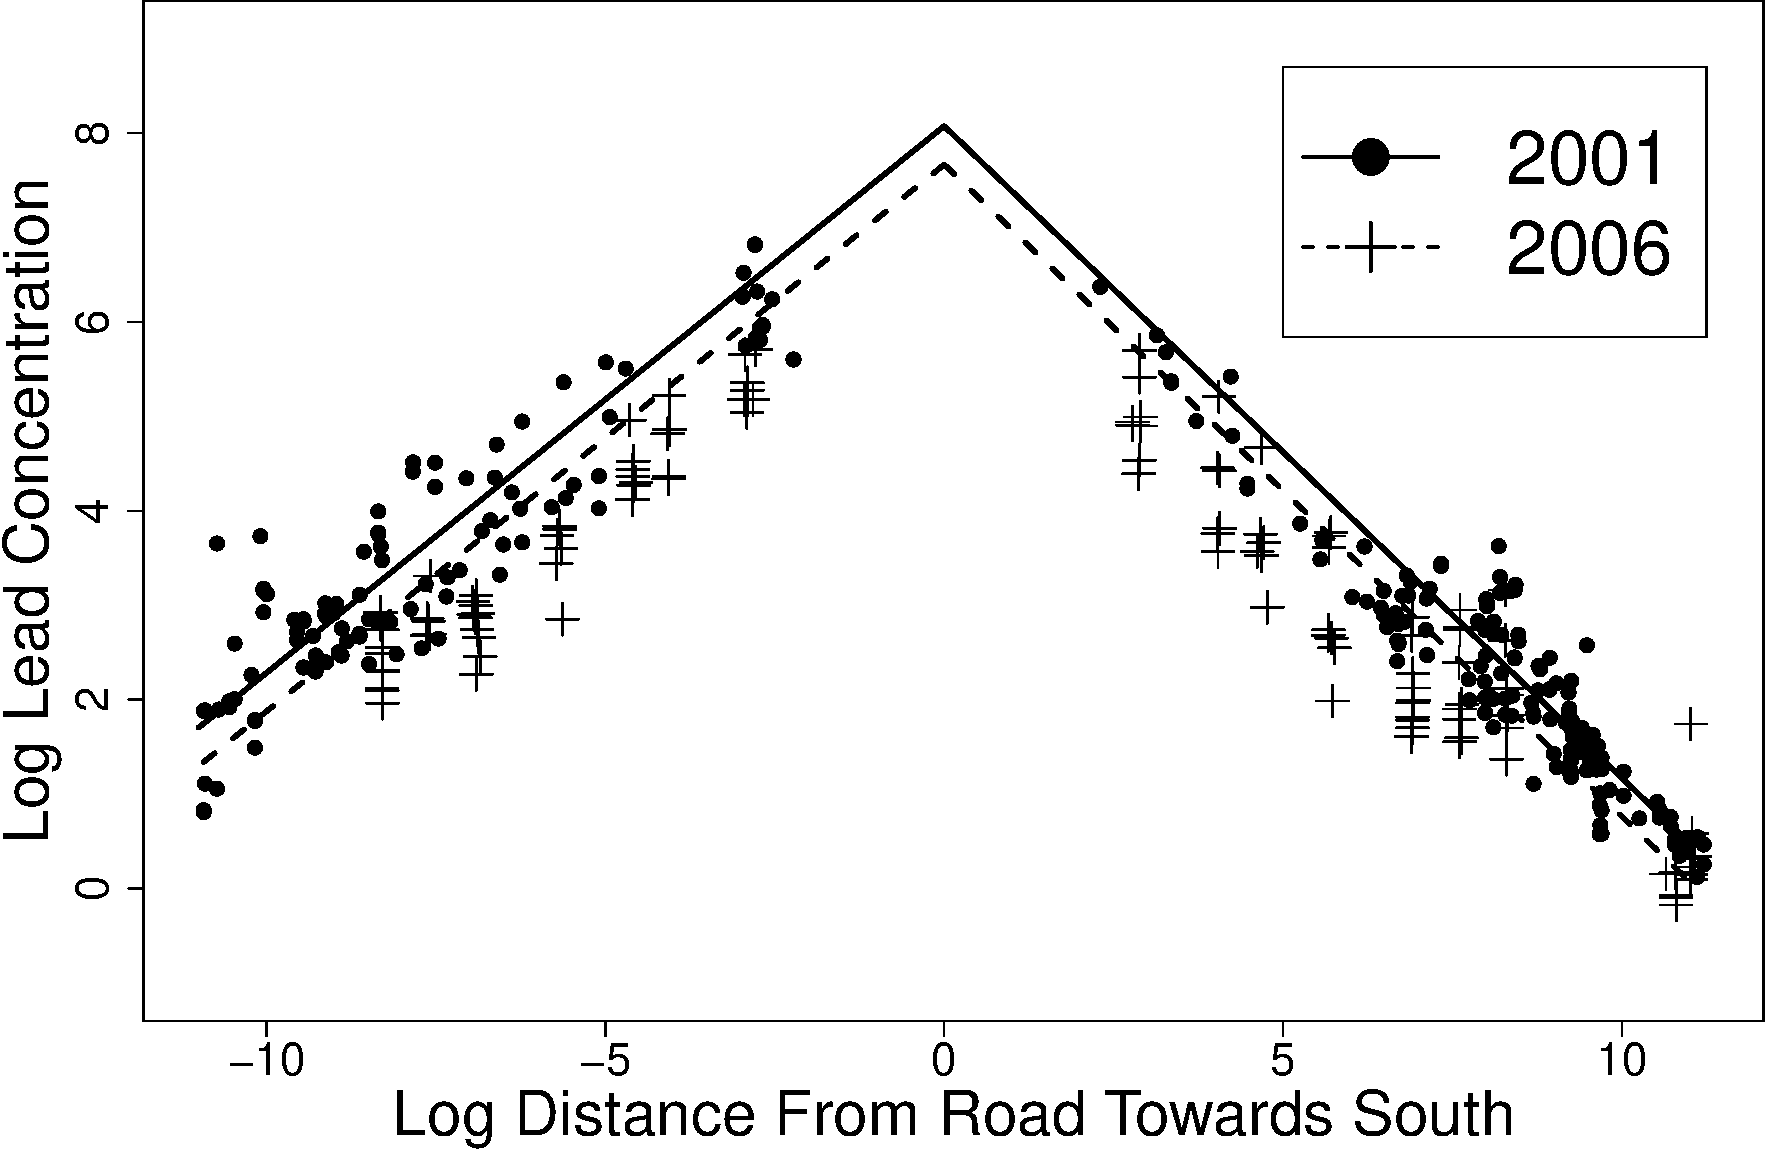
\includegraphics[width=0.9\linewidth]{Moss_modelfit}
  \end{center}
  \caption{Fitted model to moss heavy metal data.  \label{Fig:MossModelFit}}
\end{figure}

Another noteworthy feature of Figure~\ref{Fig:MossModelFit} is that the fitted line for 2006 on the north side of the road does not seem to be particularly good, as it is above most of the raw data.  What is going on here?  This is a good example of a behavior of spatial models that needs to be understood if one is to use these models.  To help clarify, we simplify the situation to 1-dimension in Figure~\ref{Fig:MossDishSim}A, where we simulated data with a bowl-shaped pattern along the single x-coordinate.  If we fit a spatial model to these data, using REMLE with an exponential autocovariance function, we obtain estimates where the range is 86.9, the partial sill is 121.2, and the nugget effect is 0.215.  This represents very strong autocorrelation, where the range and partial sill are far beyond the bounds of the x-coordinate and data, respectively.  This is not unusual, as we have seen the strong ridge in the likelihood between the partial sill and range parameter before (e.g., Figures 8.4AB, and 8.11C), where the optimum can be well beyond the bounds of the data.

If $\hat{\boldsymbol{\Sigma}}$ is the fitted covariance matrix for the data in Figure~\ref{Fig:MossDishSim}A, then the generalized least squares estimate of the overall mean, in common to all random variables that produced the data, is
$$
\hat{\mu} = \frac{\mathbf{1}^{T}\hat{\boldsymbol{\Sigma}}^{-1}\mathbf{y}}{\mathbf{1}^{T}\hat{\boldsymbol{\Sigma}}^{-1}\mathbf{1}},
$$
which for these data is $\hat{\mu} = 5.01$, and is shown as a dashed line across Figure~\ref{Fig:MossDishSim}A.  The weights applied to each datum are given directly below, Figure~\ref{Fig:MossDishSim}B, where the weights are computed as $
\mathbf{w} = (\mathbf{1}^{T}\hat{\boldsymbol{\Sigma}}^{-1})/(\mathbf{1}^{T}\hat{\boldsymbol{\Sigma}}^{-1}\mathbf{1})$.  There a two ways to understand Figure~\ref{Fig:MossDishSim}.  From an intuitive standpoint, autocorrelated data in time or space often ``run away'' from the mean for extended time and distances, producing an oscillating pattern.  However, if the covariance is proper (positive definite), then the data always return towards the mean.  If we assume that the data in Figure~\ref{Fig:MossDishSim}A are spatially autocorrelated, then it makes sense, based on the shape of the data, that they are turning toward the mean at the endpoints.  In that sense, the estimate of the mean is reasonable.  Turning to Figure~\ref{Fig:MossDishSim}B, note that the weights at the edges are largest.  If we think about ``information'', then the data in the middle are highly redundant, being autocorrelated with many of their neighbors, while the data at the edges are most independent from all other data, being the most distant from all others.  Weighting for the mean, then, puts a premium on locations that are most independent, and gives them higher weights. Note that, after estimating the spatial covariance matrix (or assuming that it is known or fixed), the weights do not depend on the data.  The weights would be the same for any set of data, such as a trending set, or an inverted bowl shape. From both an intuitive idea of returning towards the mean, or an understanding of autocorrelation and weighting, the GLS estimate of the mean makes sense.  

This simple example (Figure~\ref{Fig:MossDishSim}) also illustrates that, for spatial models, residuals \textit{do not} sum to zero.  This is important to keep in mind when performing model diagnostics, as many are computed on residuals.  Model diagnostics developed for residuals where the model is assumed to have independent errors may behave differently for spatially autocorrelated errors.

Returning to Figure~\ref{Fig:MossModelFit}, it does appear that the residuals for 2006 on the north side of the road have a somewhat bowl-shaped pattern and the same is true for the south side of the road.  The same is not true for 2001.  One might argue that the intercept for the north side of the road is tied to the intercept for the south side of the road, which complicates the interpretation.  This is true, but the model could have allowed for separate intercepts and slopes for all year by side-of-road combinations.  We leave it as an exercise for the reader to determine if the apparent fits in 2006 improve under those conditions.  Another possibility would be to add a quadratic term to distance-from-road, but it appears that would only improve the fit to 2006 on the north side of the road at the expense of more model complexity.  The current fitted model is perfectly capable and reasonable for the observed data, especially once we understand some behaviors on the way that these models are fit.

\begin{figure}[H]
  \begin{center}
	    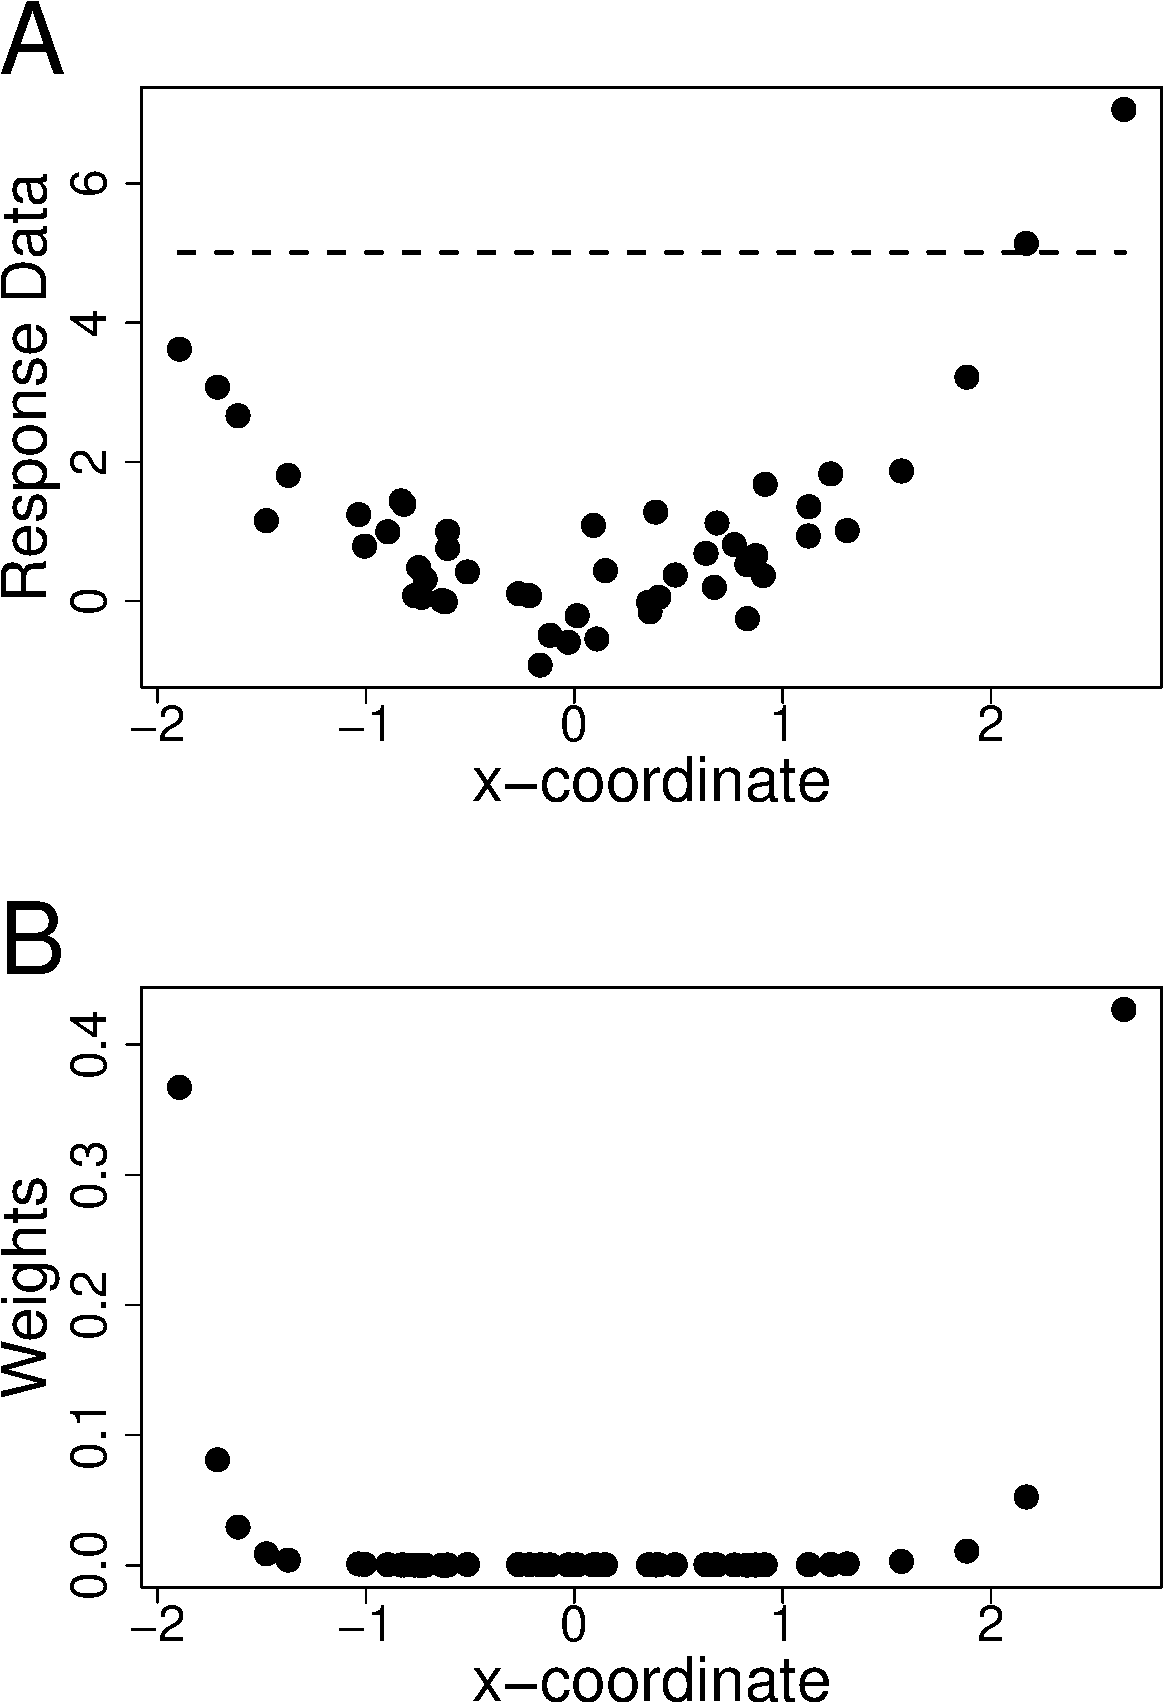
\includegraphics[width=0.6\linewidth]{Moss_dishsim}
  \end{center}
  \caption{Simulated data with bowl-shaped pattern.  A. Simulated data along a single x-coordinate, where the dashed line is the estimated mean.  B.  The weights used to compute the mean as a function of the x-coordinate of the datum.  \label{Fig:MossDishSim}}
\end{figure}

%%%%%%%%%%%%%%%%%%%%%%%%%%%%%%%%%%%%%%%%%%%%%%%%%%%%%%%%%%%%%%%%%%%%%%%%%%%%%%%%
%%%%%%%%%%%%%%%%%%%%%%%%%%%%%%%%%%%%%%%%%%%%%%%%%%%%%%%%%%%%%%%%%%%%%%%%%%%%%%%%                BIBLIOGRAPHY
%%%%%%%%%%%%%%%%%%%%%%%%%%%%%%%%%%%%%%%%%%%%%%%%%%%%%%%%%%%%%%%%%%%%%%%%%%%%%%%%
%%%%%%%%%%%%%%%%%%%%%%%%%%%%%%%%%%%%%%%%%%%%%%%%%%%%%%%%%%%%%%%%%%%%%%%%%%%%%%%%

%\bibliographystyle{consbiol}
\bibliographystyle{/mnt/ExtraDrive1/Work/shTex/asa}
\bibliography{DaleChap884.bib}
%\bibliographystyle{/home/jay/Data/shTex/shTex/asa}
%\bibliography{/home/jay/Data/shTex/shTex/StatBibTex.bib}




\end{document}

